% Options for packages loaded elsewhere
\PassOptionsToPackage{unicode}{hyperref}
\PassOptionsToPackage{hyphens}{url}
%
\documentclass[
  man]{apa6}
\usepackage{amsmath,amssymb}
\usepackage{iftex}
\ifPDFTeX
  \usepackage[T1]{fontenc}
  \usepackage[utf8]{inputenc}
  \usepackage{textcomp} % provide euro and other symbols
\else % if luatex or xetex
  \usepackage{unicode-math} % this also loads fontspec
  \defaultfontfeatures{Scale=MatchLowercase}
  \defaultfontfeatures[\rmfamily]{Ligatures=TeX,Scale=1}
\fi
\usepackage{lmodern}
\ifPDFTeX\else
  % xetex/luatex font selection
\fi
% Use upquote if available, for straight quotes in verbatim environments
\IfFileExists{upquote.sty}{\usepackage{upquote}}{}
\IfFileExists{microtype.sty}{% use microtype if available
  \usepackage[]{microtype}
  \UseMicrotypeSet[protrusion]{basicmath} % disable protrusion for tt fonts
}{}
\makeatletter
\@ifundefined{KOMAClassName}{% if non-KOMA class
  \IfFileExists{parskip.sty}{%
    \usepackage{parskip}
  }{% else
    \setlength{\parindent}{0pt}
    \setlength{\parskip}{6pt plus 2pt minus 1pt}}
}{% if KOMA class
  \KOMAoptions{parskip=half}}
\makeatother
\usepackage{xcolor}
\usepackage{graphicx}
\makeatletter
\def\maxwidth{\ifdim\Gin@nat@width>\linewidth\linewidth\else\Gin@nat@width\fi}
\def\maxheight{\ifdim\Gin@nat@height>\textheight\textheight\else\Gin@nat@height\fi}
\makeatother
% Scale images if necessary, so that they will not overflow the page
% margins by default, and it is still possible to overwrite the defaults
% using explicit options in \includegraphics[width, height, ...]{}
\setkeys{Gin}{width=\maxwidth,height=\maxheight,keepaspectratio}
% Set default figure placement to htbp
\makeatletter
\def\fps@figure{htbp}
\makeatother
\setlength{\emergencystretch}{3em} % prevent overfull lines
\providecommand{\tightlist}{%
  \setlength{\itemsep}{0pt}\setlength{\parskip}{0pt}}
\setcounter{secnumdepth}{-\maxdimen} % remove section numbering
% Make \paragraph and \subparagraph free-standing
\ifx\paragraph\undefined\else
  \let\oldparagraph\paragraph
  \renewcommand{\paragraph}[1]{\oldparagraph{#1}\mbox{}}
\fi
\ifx\subparagraph\undefined\else
  \let\oldsubparagraph\subparagraph
  \renewcommand{\subparagraph}[1]{\oldsubparagraph{#1}\mbox{}}
\fi
\newlength{\cslhangindent}
\setlength{\cslhangindent}{1.5em}
\newlength{\csllabelwidth}
\setlength{\csllabelwidth}{3em}
\newlength{\cslentryspacingunit} % times entry-spacing
\setlength{\cslentryspacingunit}{\parskip}
\newenvironment{CSLReferences}[2] % #1 hanging-ident, #2 entry spacing
 {% don't indent paragraphs
  \setlength{\parindent}{0pt}
  % turn on hanging indent if param 1 is 1
  \ifodd #1
  \let\oldpar\par
  \def\par{\hangindent=\cslhangindent\oldpar}
  \fi
  % set entry spacing
  \setlength{\parskip}{#2\cslentryspacingunit}
 }%
 {}
\usepackage{calc}
\newcommand{\CSLBlock}[1]{#1\hfill\break}
\newcommand{\CSLLeftMargin}[1]{\parbox[t]{\csllabelwidth}{#1}}
\newcommand{\CSLRightInline}[1]{\parbox[t]{\linewidth - \csllabelwidth}{#1}\break}
\newcommand{\CSLIndent}[1]{\hspace{\cslhangindent}#1}
\ifLuaTeX
\usepackage[bidi=basic]{babel}
\else
\usepackage[bidi=default]{babel}
\fi
\babelprovide[main,import]{english}
% get rid of language-specific shorthands (see #6817):
\let\LanguageShortHands\languageshorthands
\def\languageshorthands#1{}
% Manuscript styling
\usepackage{upgreek}
\captionsetup{font=singlespacing,justification=justified}

% Table formatting
\usepackage{longtable}
\usepackage{lscape}
% \usepackage[counterclockwise]{rotating}   % Landscape page setup for large tables
\usepackage{multirow}		% Table styling
\usepackage{tabularx}		% Control Column width
\usepackage[flushleft]{threeparttable}	% Allows for three part tables with a specified notes section
\usepackage{threeparttablex}            % Lets threeparttable work with longtable

% Create new environments so endfloat can handle them
% \newenvironment{ltable}
%   {\begin{landscape}\centering\begin{threeparttable}}
%   {\end{threeparttable}\end{landscape}}
\newenvironment{lltable}{\begin{landscape}\centering\begin{ThreePartTable}}{\end{ThreePartTable}\end{landscape}}

% Enables adjusting longtable caption width to table width
% Solution found at http://golatex.de/longtable-mit-caption-so-breit-wie-die-tabelle-t15767.html
\makeatletter
\newcommand\LastLTentrywidth{1em}
\newlength\longtablewidth
\setlength{\longtablewidth}{1in}
\newcommand{\getlongtablewidth}{\begingroup \ifcsname LT@\roman{LT@tables}\endcsname \global\longtablewidth=0pt \renewcommand{\LT@entry}[2]{\global\advance\longtablewidth by ##2\relax\gdef\LastLTentrywidth{##2}}\@nameuse{LT@\roman{LT@tables}} \fi \endgroup}

% \setlength{\parindent}{0.5in}
% \setlength{\parskip}{0pt plus 0pt minus 0pt}

% Overwrite redefinition of paragraph and subparagraph by the default LaTeX template
% See https://github.com/crsh/papaja/issues/292
\makeatletter
\renewcommand{\paragraph}{\@startsection{paragraph}{4}{\parindent}%
  {0\baselineskip \@plus 0.2ex \@minus 0.2ex}%
  {-1em}%
  {\normalfont\normalsize\bfseries\itshape\typesectitle}}

\renewcommand{\subparagraph}[1]{\@startsection{subparagraph}{5}{1em}%
  {0\baselineskip \@plus 0.2ex \@minus 0.2ex}%
  {-\z@\relax}%
  {\normalfont\normalsize\itshape\hspace{\parindent}{#1}\textit{\addperi}}{\relax}}
\makeatother

% \usepackage{etoolbox}
\makeatletter
\patchcmd{\HyOrg@maketitle}
  {\section{\normalfont\normalsize\abstractname}}
  {\section*{\normalfont\normalsize\abstractname}}
  {}{\typeout{Failed to patch abstract.}}
\patchcmd{\HyOrg@maketitle}
  {\section{\protect\normalfont{\@title}}}
  {\section*{\protect\normalfont{\@title}}}
  {}{\typeout{Failed to patch title.}}
\makeatother

\usepackage{xpatch}
\makeatletter
\xapptocmd\appendix
  {\xapptocmd\section
    {\addcontentsline{toc}{section}{\appendixname\ifoneappendix\else~\theappendix\fi\\: #1}}
    {}{\InnerPatchFailed}%
  }
{}{\PatchFailed}
\keywords{cognitive aging, Rescorla Wagner, spreading activation, network science, }
\DeclareDelayedFloatFlavor{ThreePartTable}{table}
\DeclareDelayedFloatFlavor{lltable}{table}
\DeclareDelayedFloatFlavor*{longtable}{table}
\makeatletter
\renewcommand{\efloat@iwrite}[1]{\immediate\expandafter\protected@write\csname efloat@post#1\endcsname{}}
\makeatother
\usepackage{lineno}

\linenumbers
\usepackage{csquotes}
\ifLuaTeX
  \usepackage{selnolig}  % disable illegal ligatures
\fi
\IfFileExists{bookmark.sty}{\usepackage{bookmark}}{\usepackage{hyperref}}
\IfFileExists{xurl.sty}{\usepackage{xurl}}{} % add URL line breaks if available
\urlstyle{same}
\hypersetup{
  pdftitle={An enrichment account of cognitive aging},
  pdfauthor={Thomas Hills1},
  pdflang={en-EN},
  pdfkeywords={cognitive aging, Rescorla Wagner, spreading activation, network science,},
  hidelinks,
  pdfcreator={LaTeX via pandoc}}

\title{An enrichment account of cognitive aging}
\author{Thomas Hills\textsuperscript{1}}
\date{}


\shorttitle{Enrichment and cognitive aging}

\authornote{

This work was supported by the Alan Turing Institute and Royal Society Wolfson Research Merit Award WM160074.

Correspondence concerning this article should be addressed to Thomas Hills, Gibbet Hill Road, Coventry, CV4 7AL, UK. E-mail: \href{mailto:t.t.hills@warwick.ac.uk}{\nolinkurl{t.t.hills@warwick.ac.uk}}

}

\affiliation{\vspace{0.5cm}\textsuperscript{1} University of Warwick}

\abstract{%
Late-life cognitive development is associated with a decline in fluid intelligence which occurs alongside a corresponding increase in crystallized intelligence.
Theory often treats these accounts independently---seeing the former as a consequence of biological aging and the latter as a natural consequence of learning. What has not been formally explored is that the lifelong learning may explain both accounts. This article describes a formal enrichment account of learning across the lifespan that shows how standard reinforcement learning exposed to a lifetime of associative learning can produce two quantitative effects recently described for cognitive aging: with age, free associations become less predictable (higher entropy) and similarity judgments fall.
The enrichment account assumes that individuals learn a cognitive representation through repeated experience with a structured environment. They then sample from that representation using spreading activation to produce associates and make similarity judgements. This reliably produces produces rising entropy and falling similarity judgments across a range of possible network types and learning assumptions. Moreover, as measures of co-activation, rising entropy and falling similarity provide mechanisms for cognitive slowing. Thus, the enrichment account shows how crystallized intelligence and fluid intelligence are intertwined and both consequences of an enriched cognitive representation.
}



\begin{document}
\maketitle

Cognitive aging across the adult lifespan is characterized by two distinct and well-document patterns. As individuals age measures of working memory, processing speed, and long-term memory show apparent performance decrements from approximately the age of 20, while at the same time, measures of vocabulary and other kinds of general knowledge increase (Park \& Reuter-Lorenz, 2009; Salthouse, 2004). This distinction between the ability to solve novel problems in a fast and accurate way, called \emph{fluid intelligence}, and the quantity of one's prior knowledge, called \emph{crystallized intelligence}, is a classic division of intelligence (Cattell, 1987). This division also stereotypically distinguishes the old from the young. What explains these age-related changes? Two prominent accounts have been proposed.

\hypertarget{degradation-and-enrichment}{%
\section{Degradation and enrichment}\label{degradation-and-enrichment}}

Declines in fluid intelligence are often seen as independent of rising crystallized intelligence. For example, the common cause theory of age-related cognitive decline argues that biological aging in the brain is the source of processing speed deficits (Deary et al., 2009). The supposition is that aging is a general process of degradation, in which factors like oxidative stress and telomere shortening damage the physiological mechanisms underpinning cognitive performance. Salthouse (1992) illustrates some potential mechanisms: ``a slower speed of transmission along single (e.g., loss of myelination) or multiple (e.g., loss of functional cells dictating circuitous linkages) pathways, or. . . delayed propagation at the connections between neural units (e.g., impairment in functioning of neurotransmitters, reduced synchronization of activation patterns)'' (p.~116). Consistent with this, percent volume of grey and white-matter declines in late life (Ge et al., 2002; Giorgio et al., 2010). Cortical thickness also declines alongside increases in cerebrospinal fluid space (Lemaitre et al., 2012). These findings are often associated with atrophy and fit with common intuitions for biological aging---things fall apart. Moreover, neuropathology---associated with posthumously verified evidence of Alzheimer's and other neurodegenerative and cerebrovascular disease---accounts for up to 40\% of the variation in late-life cognitive decline (Boyle et al., 2021). Though this leaves substantial variance in cognitive-decline unexplained, it nonetheless identifies an important correspondence between biology and cognition.

Alternatively, several accounts of cognitive aging have proposed various pathways for an interdependence between crystallized and fluid intelligence. Buchler and Reder (2007) showed using simulations that if the number of relations between concepts increased over the lifespan this would lead to more diffuse activation between concepts, analogous to a contextual fan effect. This they argued could reproduce age-related changes in recognition and familiarity. Though Buchler and Reder (2007) assumed that associations would increase, Ramscar, Hendrix, Shaoul, Milin, and Baayen (2014) used a learning model to demonstrate how associations would change through repeated learning. They based their work on Desrosiers and Ivison (1986) study of paired-associate learning in older adults, which found that older adults perform most poorly on stimuli that are least consistent with their prior experience. Ramscar, Sun, Hendrix, and Baayen (2017) showed that the difficulty of learning unrelated word pairs is entirely predictable from the frequency of co-occurrence of those words. Training a Rescorla-Wagner model on typical patterns of word co-occurrences, unrelated word pairs become negatively associated over time, which would impair learning of these concepts later.

Still more recent work has argued for a much broader influence of age-related mental `clutter', which may arise from representational changes across the lifespan as well as changes in executive function at the time of encoding or retrieval (Amer, Wynn, \& Hasher, 2022). According to this account, processing deficits and the inability to filter out past experience can lead older adults to attend to too much information. This in turn creates processing difficulties because some of this information is irrelevant, but also offers older adults benefits when `irrelevant' information becomes relevant.

The different accounts describe above can be broadly categorized as degradation versus enrichment accounts, and the evidence for both is compelling. However, to what extent we subscribe to one explanation over another is largely dependent on our understanding how these mechanisms might work. To my knowledge, the atrophy accounts have not provided formal computational mechanisms for how degradation might lead to the observed age-related changes in healthy individuals. Presumably such mechanisms could be developed and would offer useful predictions. For example, Borge-Holthoefer, Moreno, and Arenas (2011) have developed a compelling model of degradation for hyper-priming in Alzheimer's patients. In addition, formal degradation models would need to explain how these mechanisms alter fluid intelligence but not crystallized intelligence. On the other hand, enrichment explanations either assume more connectivity (e.g., Buchler and Reder (2007)) or evaluate how differential experience impairs or enhances pair-wise associations (e.g., Ramscar et al. (2014)). As called for elsewhere (Wulff, De Deyne, Jones, \& Mata, 2019), what is lacking in both cases is a full model of representational development across the adult lifespan that takes into account our understanding of the aging lexicon. This could in turn be used as a computational benchmark for understanding what we should expect from enrichment alone and what remains to be explained by degradation. In particular, two recent findings offer themselves as challenges.

\hypertarget{entropy-and-similarity-in-the-aging-lexicon}{%
\section{Entropy and similarity in the aging lexicon}\label{entropy-and-similarity-in-the-aging-lexicon}}

Several efforts to chart the mental lexicon across the lifespan using free associates have revealed reproducible trends in late life. Dubossarsky, De Deyne, and Hills (2017) asked over 8000 people, ranging in age from roughly 10 to 70, to provide three free associates to each of 420 words. With approximately 1000 people in each age group, data was aggregated within age-groups to produce networks among the 420 words with edges representing a weighted function of common associates. After thresholding the networks by removing edges below a threshold value, older networks were found to have a lower average degree (number of associations per word) and higher average shortest path length (greater distance between associates). Notably, this was underpinned by a rising entropy for associations, such that associations became less predictable across the lifespan. Zortea, Menegola, Villavicencio, and Salles (2014) found a similar pattern with a smaller group of participants. With a still smaller group of participants (n=8) but far more cues (n=3000), Wulff, De Deyne, Aeschbach, and Mata (2022) found this pattern yet again.

Analyses of memory search in older and younger adults also find consistent patterns of change in aging mental lexicons. Using a semantic fluency task (``name all the animals you can think of''), Wulff, De Deyne, et al. (2022) constructed lexical networks by connecting words that appeared nearby in the lists that older and younger adults produced and found that older adults' lexicons were less well-connected. Similarly, Hills, Mata, Wilke, and Samanez-Larkin (2013) modeled the semantic fluency task using semantic space models and found that, compared with younger adults, older adults produced strings of less similar words. Finally, Cosgrove, Kenett, Beaty, and Diaz (2021) used percolation analysis to investigate the resilience of older adults' mental lexicons by artificially removing connections between words and found that older adults' lexicons were less resilient to decay. These findings are all suggestive of more sparse connectivity in the outputs retrieved from the mental lexicon.

Judgements of similarity between words are equally consistent with the above patterns. Compared with younger adults, older adults judge animals to be less similar to one another. Wulff, Hills, and Mata (2022) asked younger and older adults to judge the similarity of 77 different animals over a period of several weeks using a tablet participants could take home with them. Rating the similarity of pairs of animals on a scale from 1 to 20, Wulff, Hills, et al. (2022) found that older adults tended to rate animals as less similar than young adults.

The key take-away with respect to what follows is that older adults produce less predictable associations (higher entropy) and lower similarity judgments than younger adults. These results are intuitively consistent with representational degradation, as we may imagine that a sparseness in output reflects a sparseness in the underlying representation. However, without understanding what we might expect from lifelong learning, efforts to explain cognitive aging as the result of degradation may attempt to bridge an explanatory gap that does not exist. Moreover, they may even get the causation backwards. Which is to say, if life experience gives rise to some of the primary markers of age-related cognitive decline, then so-called atrophy in physiological structure may not be the cause of age-related cognitive decline, but the consequence of life-long learning. As demonstrated below, by extending standard learning and retrieval models across the lifespan, we can predict both of these effects as a consequence of enrichment, without the need for assuming any additional processes associated with biological aging or degradation.

\hypertarget{the-enrichment-model}{%
\section{The enrichment model}\label{the-enrichment-model}}

The enrichment account envisions behavior as the outcome of learning relationships from the environment to develop a cognitive representation, and then using this representation to generate behavior. This follows calls from previous researchers to model not only the representation but the processes by which that representation are accessed (Estes, 1975; Johns, Jamieson, \& Jones, 2023; Jones, Hills, \& Todd, 2015). Thus, the enrichment account involves modeling three separate components:

\begin{enumerate}
\def\labelenumi{\arabic{enumi}.}
\tightlist
\item
  \emph{Environment}: The environment presents the set of possible experiences, i.e., associations.
\item
  \emph{Representation}: Learning from the environment generates a cognitive representation. This continues to develop across the lifespan.
\item
  \emph{Behavior}: Behavior is recovery of information from the cognitive representation appropriate to the environmental context. This generates free-associations, memory search, similarity judgments, and so on.
\end{enumerate}

These stages are presented in Figure \ref{fig:Figure1} and each are explained in detail below.

\begin{figure}
\centering
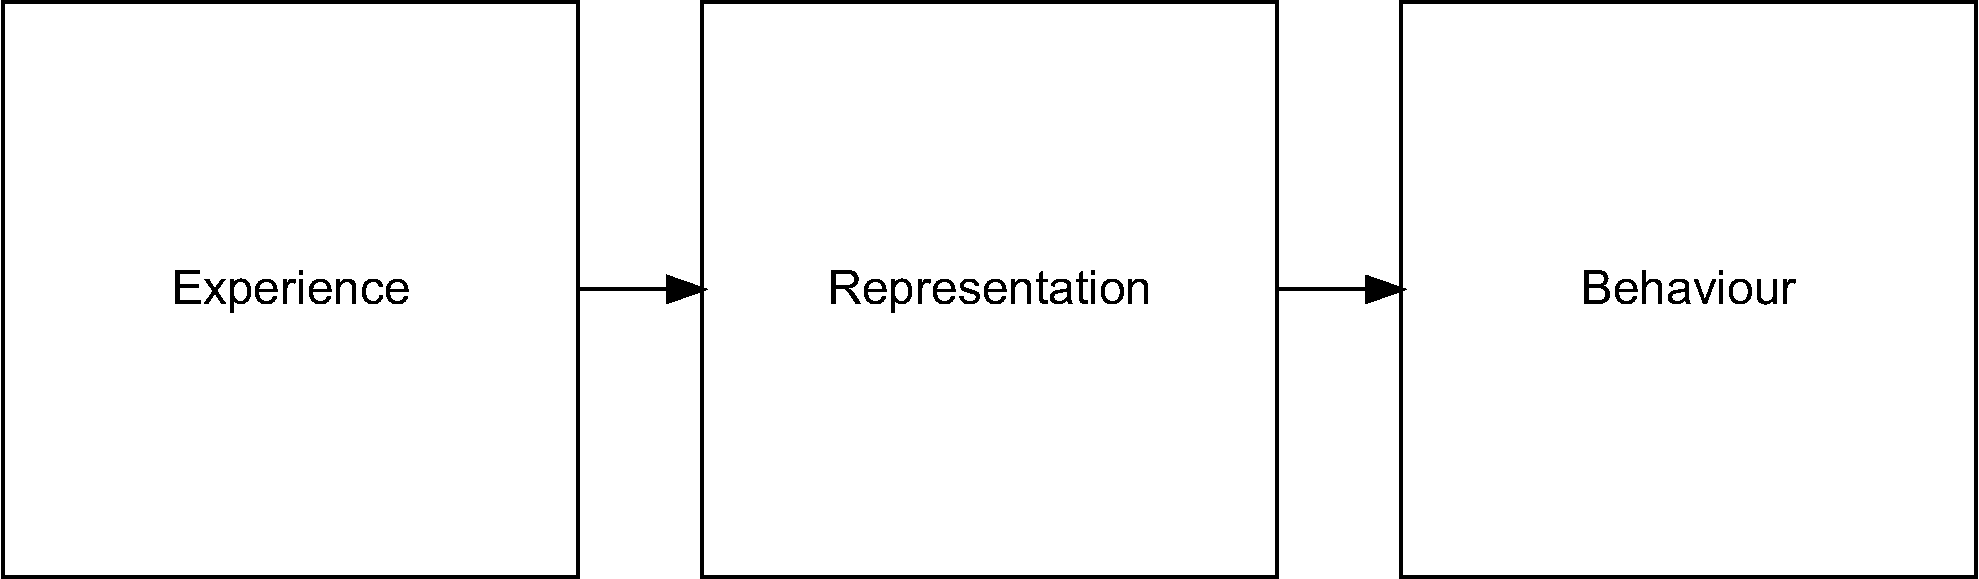
\includegraphics{Enrichment_files/figure-latex/Figure1-1.pdf}
\caption{\label{fig:Figure1}The process of translating environmental experiences into behaviour. Arrows represent processes that translate one domain into another. Learning translates experience into a cognitive representation. Additional cognitive processes then act on the representation to generate behavior.}
\end{figure}

\hypertarget{environment}{%
\subsection{Environment}\label{environment}}

The environment presents the set of possible relationships an individual could learn. It is represented here as network of concepts (e.g., words), with the edges between concepts indicating learnable associations. The environment presented here is a variation of fitness-based network model using rank-based sampling. This is inspired by the ubiquity of scaling laws in the cognitive sciences and the natural world (\textbf{Kello2010ga?}). This assumes a power-law relation in the frequency of concepts: Each concept is assigned a rank, \(r\), from 1 to 1000. Then pairs of concepts are chosen from the lexicon each with probability \(p \propto r^{-a}\) and an edge is created between them. Here \(a\) is set to \(.1\) and 2000 edges are created. A scale-free network is not required to get the aging results shown below---for example, an Erdös-Renyi random graph produces the same qualitative pattern. In addition, the number of words available to learn could increase across the lifespan, as proposed by Brysbaert, Stevens, Mandera, and Keuleers (2016) and following \emph{Herdan-Heaps' law} (Petersen, Tenenbaum, Havlin, Stanley, \& Perc, 2012; Serrano, Flammini, \& Menczer, 2009). Again, the qualitative results are the same. Examples are provided in the Supplementary material.

\hypertarget{representation}{%
\subsection{Representation}\label{representation}}

To build a cognitive representation from experiences with the environment, I use the basic prediction error framework set out in the Rescorla-Wagner model. This follows the strong evidence for learning as a process of minimizing prediction error, which is a fundamental assumption among models of reinforcement learning (Dayan \& Abbott, 2005; Hoppe, Hendriks, Ramscar, \& Rij, 2022; McClelland \& Rumelhart, 1981; Sutton \& Barto, 2018). The Rescorla-Wagner model (Rescorla \& Wagner, 1972) captures this phenomenology---including associative learning, blocking, inhibition, and extinction---and it is a model on which many subsequent models have been based (e.g., Sutton \& Barto, 1981; Trimmer, McNamara, Houston, \& Marshall, 2012). Though it is not without criticism (Yau \& McNally, 2023), I use the model here to capture the basic prediction-error framework inherent in its design.

Formally, the Rescorla-Wagner model minimizes the prediction error between the values of an observed outcome, \(\lambda_j\) and a cue predictive of that outcome, \(V_{i \rightarrow j}\), where \(j\) and \(i\) represent specific outcomes and cues, respectively. The prediction error is the difference between them, \((\lambda_j-V_i)\), and it is minimized following each learning event according to the following rule:

\[
\Delta V_{i \rightarrow j} = \alpha_i \beta_j (\lambda_{j} - V_{i \rightarrow j})
\]

\(\alpha_i\) corresponds to cue salience (some cues are easier to learn about than others) and \(\beta_j\) to the learning rate (some outcomes are learned about faster than others). Both \(\alpha\) and \(\beta\) values are confined to values between \(0\) and \(1\). After learning at time \(t\), the updated cue value is

\[
V_{i \rightarrow j, t+1} = V_{i \rightarrow j, t} + \Delta V_{i \rightarrow j, t}
\]

This follows the formalizations set out in prior work (Ramscar et al., 2017; Rescorla \& Wagner, 1972).

The cognitive representation is formed by applying the Rescorla-Wagner model to the environment in the following way. Each learning event randomly samples a relationship from the environment represented as an edge (or association) in the environment network. Of the two concepts at each end of the edge, one is randomly assigned as the cue and the other as the outcome. The representation is then updated according to the Rescorla-Wagner model with \(\alpha=1\) and \(\beta=.2\) and \(\lambda_i=1\).

\hypertarget{behaviour}{%
\subsection{Behaviour}\label{behaviour}}

The two stylized facts associated with cognitive aging are rising entropy and a reduction in pairwise similarity judgments. Each of these is recovered from the representation as follows.

\hypertarget{rising-entropy}{%
\subsubsection{Rising entropy}\label{rising-entropy}}

Rising entropy refers to the reduction in the predictability of free association targets as individuals age (Dubossarsky et al., 2017). We can measure this using \emph{Shannon's information entropy}. This measures the surprisingness of associates given the cue. Because the output of Rescorla-Wagner learning is a weighted edge, we can compute this for every cue in the network representation as follows:

\[
H = -\sum_{i=1}^{k}  p_i log(p_i)
\] Here, \(p_i\) is the proportion of the weight along edge \(i\) for all \(k\) edges. That is, \(p_i = \frac{w_i}{\sum_k w_k}\).

\hypertarget{similarity}{%
\subsubsection{Similarity}\label{similarity}}

To simulate similarity judgments, we create a measure of co-activation between cues. To do this, we allow spreading activation to leave one node and measuring activation at the other node, \(A_{j \rightarrow k}\). This allows us to measure the extent to which one word co-activates the other. Doing this for both cues, we take similarity as the summed co-activation.

\[
S = A_{j \rightarrow k} + A_{j \rightarrow k}
\]

We measure this similarity for all node pairs in the representation.

\hypertarget{results}{%
\section{Results}\label{results}}

\begin{verbatim}
## Warning in xy.coords(x, y, xlabel, ylabel, log): 52 y values <= 0 omitted from
## logarithmic plot
\end{verbatim}

\begin{figure}
\centering
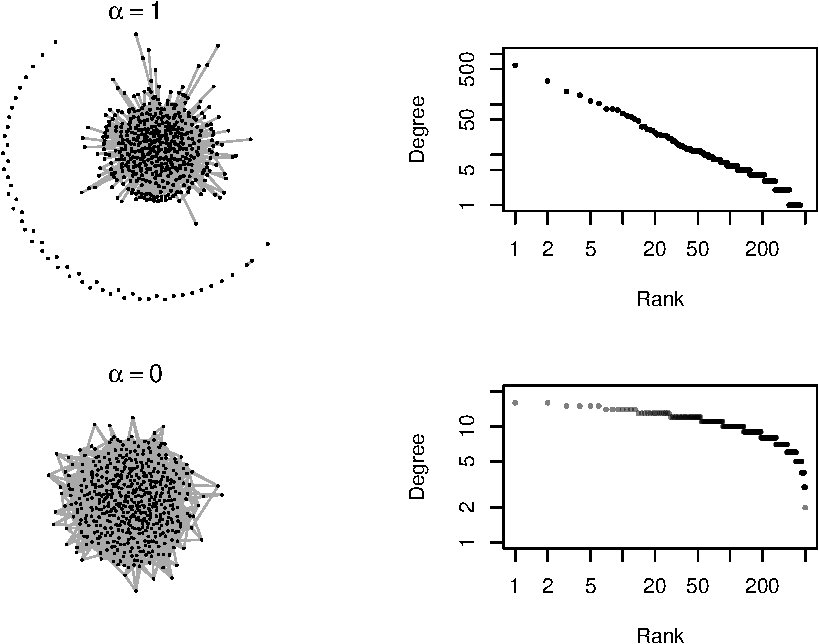
\includegraphics{Enrichment_files/figure-latex/fig1-1.pdf}
\caption{\label{fig:fig1}The structure of the environment.}
\end{figure}

\begin{figure}
\centering
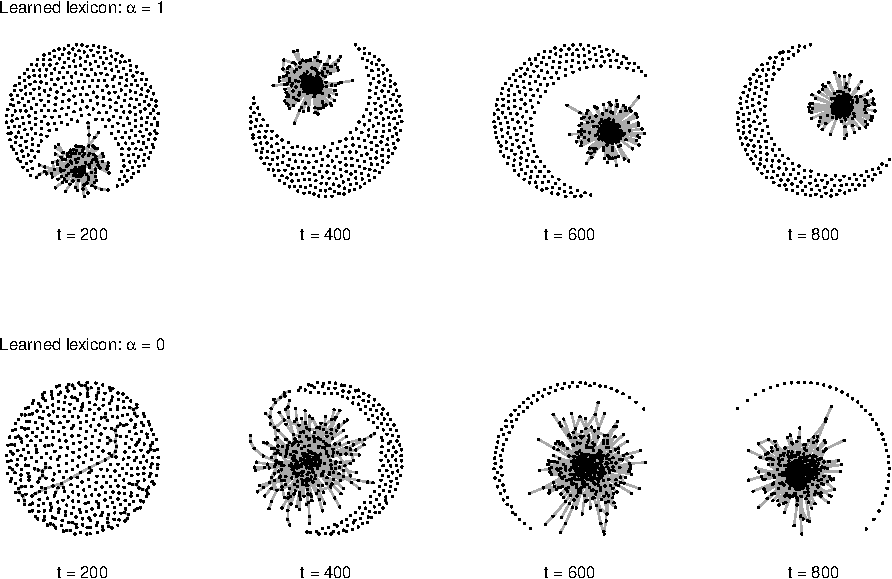
\includegraphics{Enrichment_files/figure-latex/fig2-1.pdf}
\caption{\label{fig:fig2}The growing mental lexicon.}
\end{figure}

\begin{figure}

{\centering 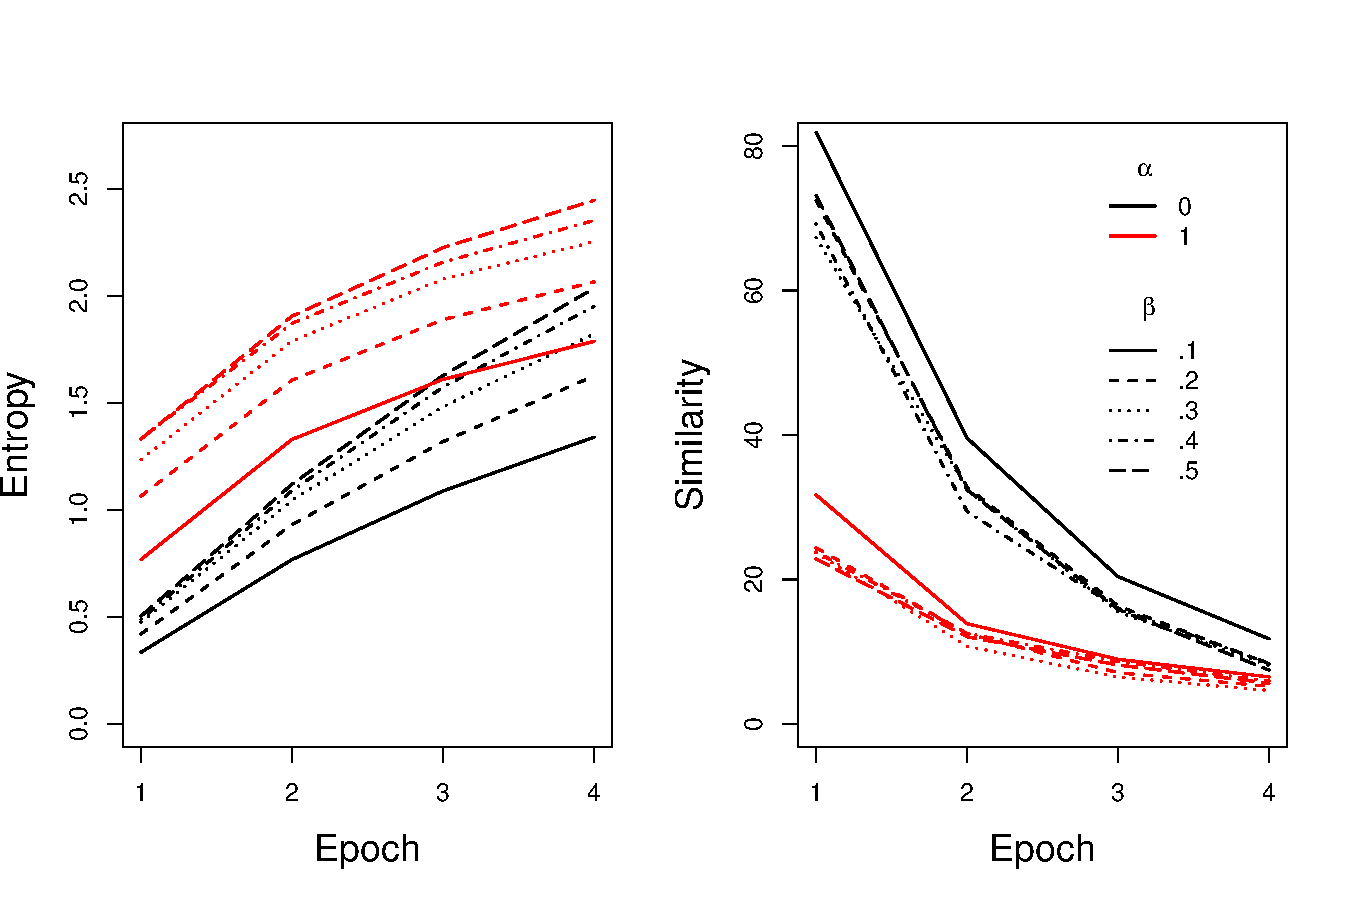
\includegraphics[width=1\linewidth]{EntropySim} 

}

\caption{Entropy and similarity measures computed from the cognitive representation at different epochs of development.}\label{fig:unnamed-chunk-1}
\end{figure}

\hypertarget{the-network-of-associations}{%
\section{The network of associations}\label{the-network-of-associations}}

As noted above, Dubossarsky et al. (2017) and others found that free association networks collected across the adult lifespan showed patterns of decreasing network degree, increasing average shortest path length, and decreasing clustering coefficient. We can simulate this on the above cognitive representations across the four epochs as follows. For each cognitive representation, we simulate 10 participants who retrieve 3 associates from each of 30 cues. The three associates are sampled without replacement for each participant and each cue in proportion to the associative strength encoded in the cognitive representation, i.e., the output from the Rescorla-Wagner training epochs. Negative association strengths are set to 0. This produces a cue by associate matrix, which each cell indicates the number of times each associate was produced in response to each cue. From this matrix, cue-by-cue similarities can be computed using cosine similarity. To transform these into unweighted and undirected networks, the median cue-by-cue similarity is computed across all epochs and then, for each age, cue similarities below this median value are set to 0, and all other values are set to 1. This matrix is then transformed into a network on which degree (the number of connections), average shortest path length (the shortest number of edges between cues), and clustering coefficient (the proportion of a node's neighbors that are themselves connected) are computed. This entire process is repeated for 50 different initial starting environments. The results are shown in Figure ???, and they follow the pattern found by Dubossarsky et al. (2017). This suggests that the results found in previous work in association with the aging lexicon could in principle be a consequence of lifelong learning.

\begin{figure}

{\centering 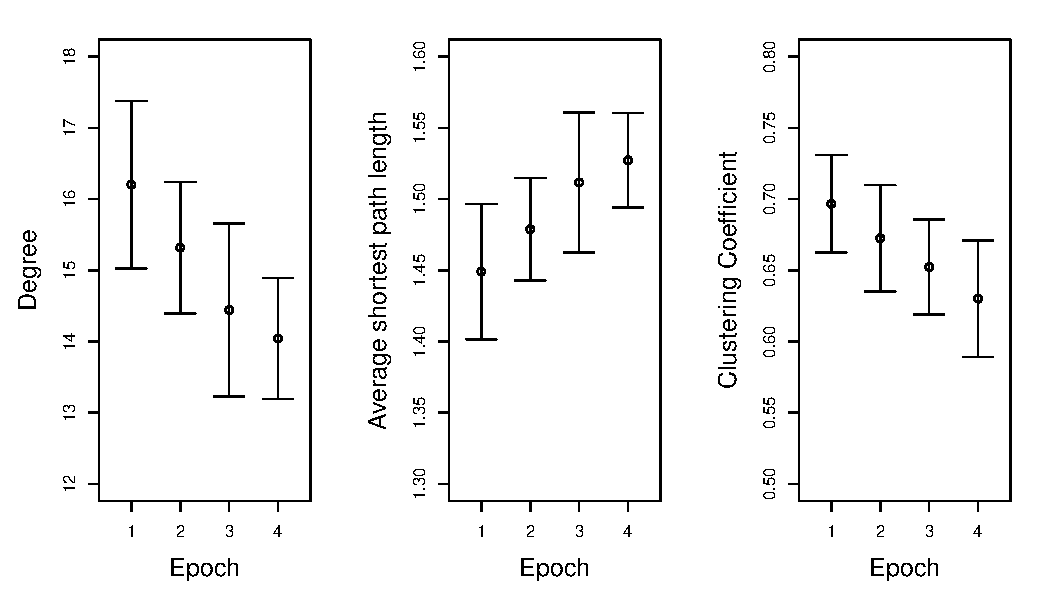
\includegraphics[width=1\linewidth]{NetworkAssociations} 

}

\caption{The degree, average shortest path length, and clustering coefficient for networks of associations across the lifespan. Simulations were repeated for learning in 100 different environments ($a=1$) with four training epochs each ($beta=.1$), as in Figure 3, which were then each sampled from by 10 simulated participants who each retrieved 3 associates for each of 30 cues with probability proportional to associative strengths output from the Rescorla-Wagner training epoch. The cosine similarity of cues was then computed on the resulting cue by associate network to produce associative networks for each epoch. These networks were then thresholded separately for each learning environment by the median similarity value across all ages. Results are consistent with Dubossarsky et al., 2017.}\label{fig:unnamed-chunk-2}
\end{figure}

\hypertarget{discussion}{%
\section{Discussion}\label{discussion}}

Because edges were formed in Dubossarsky et al. (2017) and Wulff et al. (2019) by requiring a minimun number of cue-target associations in the free association task, rising entropy corresponds to a less predictable pattern of cue-target associations and the lower likelihood of an edge between any cue-target pair. As a consequence, representational networks with higher entropy will produce behavioural networks that are more sparse.

Write some more stuff.

Do people who learn more showing earlier degradation? look at clutter paper.

Ramscar et al. (2014) suggested that ``older adults' changing performance reflects memory search demands, which escalate as experience grows'' (p.~5) because older adults largely show impaired paired-associated learning only for unrelated terms. In subsequent work,

Borges-holthoefer hyperpriming (the opposite effect)

What do we mean by learning? We don't mean higher education.

As the authors note, ``Experience is underappreciated as a factor in cognitive performance and is absent in most models of cognitive aging'' (p.~118).

By their account, proposing biological aging is uneccesary as the result is already explained by standard learning models. As Ramscar et al. (2017) state, ``the discriminative processes that produce `associative' learning teaches English speakers not only which words go together, but also which words do not go together. This process both increasingly differentiates meaningful and meaningless word pairs and makes meaningless pairs harder to learn'' (p.~3).

\newpage

\hypertarget{references}{%
\section{References}\label{references}}

\hypertarget{refs}{}
\begin{CSLReferences}{1}{0}
\leavevmode\vadjust pre{\hypertarget{ref-amer2022cluttered}{}}%
Amer, T., Wynn, J. S., \& Hasher, L. (2022). Cluttered memory representations shape cognition in old age. \emph{Trends in Cognitive Sciences}, \emph{26}(3), 255--267.

\leavevmode\vadjust pre{\hypertarget{ref-BorgeHolthoefer:2011bg}{}}%
Borge-Holthoefer, J., Moreno, Y., \& Arenas, A. (2011). {Modeling abnormal priming in Alzheimer's patients with a free association network}. \emph{PLoS ONE}, \emph{6}(8), e22651.

\leavevmode\vadjust pre{\hypertarget{ref-boyle2021degree}{}}%
Boyle, P. A., Wang, T., Yu, L., Wilson, R. S., Dawe, R., Arfanakis, K., \ldots{} Bennett, D. A. (2021). To what degree is late life cognitive decline driven by age-related neuropathologies? \emph{Brain}, \emph{144}(7), 2166--2175.

\leavevmode\vadjust pre{\hypertarget{ref-brysbaert2016many}{}}%
Brysbaert, M., Stevens, M., Mandera, P., \& Keuleers, E. (2016). How many words do we know? Practical estimates of vocabulary size dependent on word definition, the degree of language input and the participant's age. \emph{Frontiers in Psychology}, \emph{7}(1116), 1--11.

\leavevmode\vadjust pre{\hypertarget{ref-buchler2007modeling}{}}%
Buchler, N. E., \& Reder, L. M. (2007). Modeling age-related memory deficits: A two-parameter solution. \emph{Psychology and Aging}, \emph{22}(1), 104.

\leavevmode\vadjust pre{\hypertarget{ref-cattell1987intelligence}{}}%
Cattell, R. B. (1987). \emph{Intelligence: Its structure, growth and action}. Elsevier.

\leavevmode\vadjust pre{\hypertarget{ref-cosgrove2021quantifying}{}}%
Cosgrove, A. L., Kenett, Y. N., Beaty, R. E., \& Diaz, M. T. (2021). Quantifying flexibility in thought: The resiliency of semantic networks differs across the lifespan. \emph{Cognition}, \emph{211}, 104631.

\leavevmode\vadjust pre{\hypertarget{ref-dayan2005theoretical}{}}%
Dayan, P., \& Abbott, L. F. (2005). \emph{Theoretical neuroscience: Computational and mathematical modeling of neural systems}. MIT Press.

\leavevmode\vadjust pre{\hypertarget{ref-deary2009age}{}}%
Deary, I. J., Corley, J., Gow, A. J., Harris, S. E., Houlihan, L. M., Marioni, R. E., \ldots{} Starr, J. M. (2009). Age-associated cognitive decline. \emph{British Medical Bulletin}, \emph{92}(1), 135--152.

\leavevmode\vadjust pre{\hypertarget{ref-desrosiers1986paired}{}}%
Desrosiers, G., \& Ivison, D. (1986). Paired associate learning: Normative data for differences between high and low associate word pairs. \emph{Journal of Clinical and Experimental Neuropsychology}, \emph{8}(6), 637--642.

\leavevmode\vadjust pre{\hypertarget{ref-dubossarsky2017quantifying}{}}%
Dubossarsky, H., De Deyne, S., \& Hills, T. (2017). Quantifying the structure of free association networks across the life span. \emph{Developmental Psychology}, \emph{53}(8), 1560--1570.

\leavevmode\vadjust pre{\hypertarget{ref-estes1975some}{}}%
Estes, W. (1975). Some targets for mathematical psychology. \emph{Journal of Mathematical Psychology}, \emph{12}(3), 263--282.

\leavevmode\vadjust pre{\hypertarget{ref-ge2002age}{}}%
Ge, Y., Grossman, R. I., Babb, J. S., Rabin, M. L., Mannon, L. J., \& Kolson, D. L. (2002). Age-related total gray matter and white matter changes in normal adult brain. Part i: Volumetric MR imaging analysis. \emph{American Journal of Neuroradiology}, \emph{23}(8), 1327--1333.

\leavevmode\vadjust pre{\hypertarget{ref-giorgio2010age}{}}%
Giorgio, A., Santelli, L., Tomassini, V., Bosnell, R., Smith, S., De Stefano, N., \& Johansen-Berg, H. (2010). Age-related changes in grey and white matter structure throughout adulthood. \emph{Neuroimage}, \emph{51}(3), 943--951.

\leavevmode\vadjust pre{\hypertarget{ref-hills2013mechanisms}{}}%
Hills, T., Mata, R., Wilke, A., \& Samanez-Larkin, G. R. (2013). Mechanisms of age-related decline in memory search across the adult life span. \emph{Developmental Psychology}, \emph{49}(12), 2396--2404.

\leavevmode\vadjust pre{\hypertarget{ref-hoppe2022exploration}{}}%
Hoppe, D. B., Hendriks, P., Ramscar, M., \& Rij, J. van. (2022). An exploration of error-driven learning in simple two-layer networks from a discriminative learning perspective. \emph{Behavior Research Methods}, \emph{54}(5), 2221--2251.

\leavevmode\vadjust pre{\hypertarget{ref-johns2023scalable}{}}%
Johns, B. T., Jamieson, R. K., \& Jones, M. N. (2023). {Scalable cognitive modelling: Putting Simon's (1969) ant back on the beach.} \emph{Canadian Journal of Experimental Psychology/Revue Canadienne de Psychologie Exp{é}rimentale}, \emph{77}(3), 185--201.

\leavevmode\vadjust pre{\hypertarget{ref-jones2015hidden}{}}%
Jones, M. N., Hills, T., \& Todd, P. M. (2015). Hidden processes in structural representations: A reply to abbott, austerweil, and griffiths (2015). \emph{Psychological Review}, \emph{122}(3), 570--574.

\leavevmode\vadjust pre{\hypertarget{ref-lemaitre2012normal}{}}%
Lemaitre, H., Goldman, A. L., Sambataro, F., Verchinski, B. A., Meyer-Lindenberg, A., Weinberger, D. R., \& Mattay, V. S. (2012). Normal age-related brain morphometric changes: Nonuniformity across cortical thickness, surface area and gray matter volume? \emph{Neurobiology of Aging}, \emph{33}(3), 617--e1.

\leavevmode\vadjust pre{\hypertarget{ref-mcclelland1981interactive}{}}%
McClelland, J. L., \& Rumelhart, D. E. (1981). An interactive activation model of context effects in letter perception: I. An account of basic findings. \emph{Psychological Review}, \emph{88}(5), 375--407.

\leavevmode\vadjust pre{\hypertarget{ref-park2009adaptive}{}}%
Park, D. C., \& Reuter-Lorenz, P. (2009). The adaptive brain: Aging and neurocognitive scaffolding. \emph{Annual Review of Psychology}, \emph{60}, 173--196.

\leavevmode\vadjust pre{\hypertarget{ref-petersen2012languages}{}}%
Petersen, A. M., Tenenbaum, J. N., Havlin, S., Stanley, H. E., \& Perc, M. (2012). Languages cool as they expand: Allometric scaling and the decreasing need for new words. \emph{Scientific Reports}, \emph{2}(943), 1--10.

\leavevmode\vadjust pre{\hypertarget{ref-ramscar2014myth}{}}%
Ramscar, M., Hendrix, P., Shaoul, C., Milin, P., \& Baayen, H. (2014). The myth of cognitive decline: Non-linear dynamics of lifelong learning. \emph{Topics in Cognitive Science}, \emph{6}(1), 5--42.

\leavevmode\vadjust pre{\hypertarget{ref-ramscar2017mismeasurement}{}}%
Ramscar, M., Sun, C. C., Hendrix, P., \& Baayen, H. (2017). The mismeasurement of mind: Life-span changes in paired-associate-learning scores reflect the {``cost''} of learning, not cognitive decline. \emph{Psychological Science}, \emph{28}(8), 1171--1179.

\leavevmode\vadjust pre{\hypertarget{ref-rescorla1972theory}{}}%
Rescorla, R. A., \& Wagner, A. R. (1972). {A theory of Pavlovian conditioning: Variations in the effectiveness of reinforcement and non-reinforcement}. In A. H. Prokasy (Ed.), \emph{Classical conditioning II: Current research and theory} (pp. 64--69). Appleton-Century-Crofts.

\leavevmode\vadjust pre{\hypertarget{ref-salthouse2013mechanisms}{}}%
Salthouse, T. A. (1992). \emph{Mechanisms of age-cognition relations in adulthood}. Lawrence Erlbaum Associates, Inc.

\leavevmode\vadjust pre{\hypertarget{ref-Salthouse:2004is}{}}%
Salthouse, T. A. (2004). {What and when of cognitive aging}. \emph{Current Directions in Psychological Science}, \emph{13}(4), 140--144.

\leavevmode\vadjust pre{\hypertarget{ref-Serrano:2009cv}{}}%
Serrano, M. Á., Flammini, A., \& Menczer, F. (2009). Modeling statistical properties of written text. \emph{PLoS ONE}, \emph{4}(4), e5372.

\leavevmode\vadjust pre{\hypertarget{ref-sutton1981toward}{}}%
Sutton, R. S., \& Barto, A. G. (1981). Toward a modern theory of adaptive networks: Expectation and prediction. \emph{Psychological Review}, \emph{88}(2), 135.

\leavevmode\vadjust pre{\hypertarget{ref-sutton2018reinforcement}{}}%
Sutton, R. S., \& Barto, A. G. (2018). \emph{Reinforcement learning: An introduction}. MIT Press.

\leavevmode\vadjust pre{\hypertarget{ref-trimmer2012does}{}}%
Trimmer, P. C., McNamara, J. M., Houston, A. I., \& Marshall, J. A. (2012). Does natural selection favour the rescorla--wagner rule? \emph{Journal of Theoretical Biology}, \emph{302}, 39--52.

\leavevmode\vadjust pre{\hypertarget{ref-wulff2022using}{}}%
Wulff, D. U., De Deyne, S., Aeschbach, S., \& Mata, R. (2022). Using network science to understand the aging lexicon: Linking individuals' experience, semantic networks, and cognitive performance. \emph{Topics in Cognitive Science}, \emph{14}(1), 93--110.

\leavevmode\vadjust pre{\hypertarget{ref-wulff2019new}{}}%
Wulff, D. U., De Deyne, S., Jones, M. N., \& Mata, R. (2019). New perspectives on the aging lexicon. \emph{Trends in Cognitive Sciences}, \emph{23}(8), 686--698.

\leavevmode\vadjust pre{\hypertarget{ref-wulff2022structural}{}}%
Wulff, D. U., Hills, T., \& Mata, R. (2022). Structural differences in the semantic networks of younger and older adults. \emph{Scientific Reports}, \emph{12}(21459), 1--13.

\leavevmode\vadjust pre{\hypertarget{ref-yau2023rescorla}{}}%
Yau, J. O.-Y., \& McNally, G. P. (2023). The rescorla-wagner model, prediction error, and fear learning. \emph{Neurobiology of Learning and Memory}, \emph{203}, 107799.

\leavevmode\vadjust pre{\hypertarget{ref-zortea2014graph}{}}%
Zortea, M., Menegola, B., Villavicencio, A., \& Salles, J. F. de. (2014). Graph analysis of semantic word association among children, adults, and the elderly. \emph{Psicologia: Reflexao e Critica}, \emph{27}, 90--99.

\end{CSLReferences}


\end{document}
